\documentclass[12pt,a4paper]{report}
\usepackage{graphicx}
\usepackage{float}
\usepackage{rotating}
\usepackage{listings}
\usepackage{color}
\usepackage{fullpage}

\lstset{ % General setup for the package
	basicstyle=\tiny\sffamily,
	numbers=left,
 	numberstyle=\tiny,
	frame=tb,
	tabsize=4,
	columns=fixed,
	showstringspaces=false,
	showtabs=false,
	keepspaces,
	commentstyle=\color{red},
	keywordstyle=\color{blue}
}

\begin{document}
\begin{titlepage}
	\centering
	
\includegraphics[width=0.15\textwidth]{img/concordia_logo.jpg}\par\vspace{1cm}
	{\scshape\LARGE Concordia University \par}
	\vspace{1cm}
	{\scshape\Large COMP 371 \par}
	\vspace{1.5cm}
	{\huge\bfseries \uppercase{Project Implementation Plan} \par}
	\vspace{1cm}
	{\huge\bfseries Interactive Museum \par}
	\vspace{2cm}
	{\Large \uppercase{\textbf{Team \#4}}\par}
	\vspace{0.5cm}
	{Patrick Olivier Jean Baptiste\par}
	{Sean O'Connor\par}
	{Arturo Santamaria Gonzalez\par}
	{Christian Galante\par}
	\vfill
	\textsc{}

	\vfill

% Bottom of the page
	{\large \today\par}
\end{titlepage}
\section*{Introduction}
\par The overall theme we have chosen to implement for the project is the \textbf{Interactive Museum}. The museum shall have four zones dedicated each to a single idea, the ideas for these four rooms will be detailed in the following sections. The viewer shall be able to interact with objects in each of the four rooms of the scene to change the respective environments and accentuate the ideas present in each of the rooms.
\section*{Implementation}
\par Although each room in the interactive museum will be distinct from each other, the overall layout of the museum will be circular such that leaving the final room brings the viewer into the first room again. Each room’s lighting and sound is isolated one from the other.
\subsection*{Room 1}
\par Upon entering the room, there will be a life-size statue in the middle of the room, illuminated by a white spotlight. The room will be dimly lit with ambient lighting which takes on the same colour as the spotlight. In front of the statue will be a button which the viewer may walk up to and press to change the colour of the spotlight. In order to implement this we would require lighting and shadow calculations using ray casting.
\begin{center}
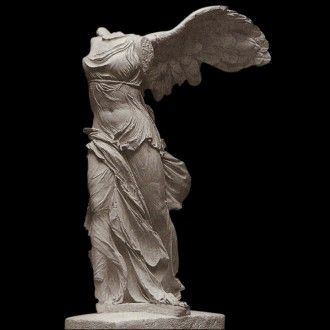
\includegraphics[scale=0.7]{img/nike.jpg}
\end{center}

\pagebreak

\subsection*{Room 2 - Sound}
\par This room has a gramophone in the center which is playing jazz music in the direction of the speaker. The viewer is able to rotate the gramophone to change the direction of the speaker. It will be necessary for this room to implement sound ray casting just as we have done for lighting in order to get across the directionality of sound using stereo speakers or headphones.
\begin{center}
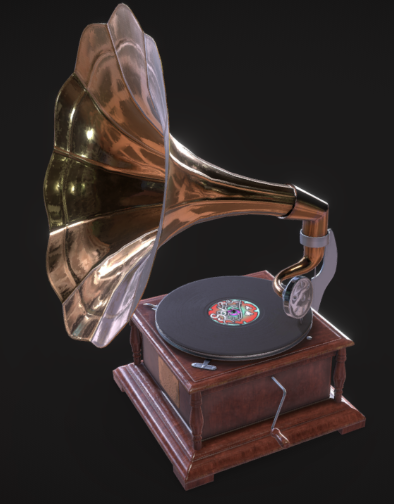
\includegraphics[scale=0.5]{img/gramophone.png}
\end{center}

\subsection*{Room 3 - Reflections/Light}
\par An object (ex: a sphere, a cube) moves about the room along straight trajectories. The object itself is either a mirror or a light source (or can be toggled between these states). As the object impacts surfaces of the room (walls, other stationary doodads) it rebounds off on a new trajectory. As the object moves we can observe how the lighting and reflections change.

\par A more advanced version might have the bouncing object acquire, transfer or swap its appearance with the surface it impacts (ex: a red sphere hits a mirrored wall, the wall becomes red, the sphere becomes mirrored)

\subsection*{Room 4 - Black Hole Simulation}
\par This room would simulate “being in a black hole”. Having a bridge from door to door, everything but the bridge itself would rotate and distort, creating a stimulating effect for the user crossing the bridge. It would be implemented by having every object but the bridge following similar transformation matrices such as a rotation matrix.

\pagebreak

\section*{Schedule}
\par The following Gantt chart details the phases of this project and our tentative time frames for completing each of these phases. This is merely a recommendation to stay on track, realistically it is possible that some phases are completed early, and therefore consequent phases will begin earlier than what is shown in the chart.
\begin{center}
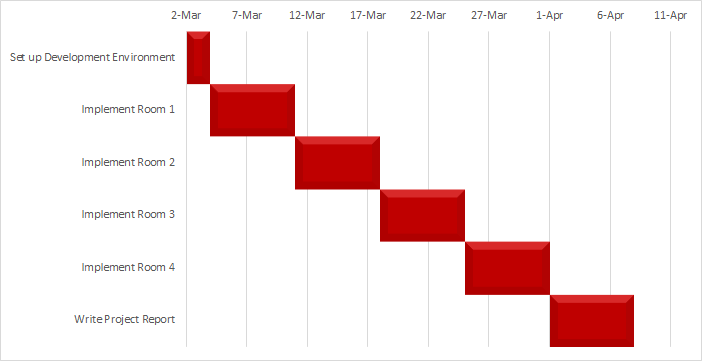
\includegraphics[width=1\textwidth]{img/schedule.png}
\end{center}
\end{document}